%Resultate für q0 von null bis 1

\subsection{Influence of the parameter $q_0$}

In figure \ref{fig:q0zushortestpath} one can observe the influence of $q_0$ on the shortest path found after 800 rounds averaged over 10 runs for the problem \textit{oliver30}. This parameter is a measure of how random the next city is chosen (see chapter \ref{sec:model}). If the model acts with a small $q_0$ the following cities are mostly chosen randomly and do not depend strongly on the amount of pheromone on the edge or the length of the edge. As one can see a $q_0$ below 0.6 leads to a path which is a few units longer then the known solution and the error gets bigger as well. Whereas $q_0$'s in the range of 0.8 to 0.95 result in a average path which lies on the known solution and the error is vanishingly small. The problem with a $q_0 = 1$ is the fact that the ants can get stuck in a strong local minimum. The 'local' shortest path gets strongly rewarded and the edges get stronger and stronger and the ants never see a reason to change their path. Therefore one needs a certain probability that one 'crazy' ant tries some new path which can lead to a new shortest path found.

\begin{figure}[H]

	\centering
	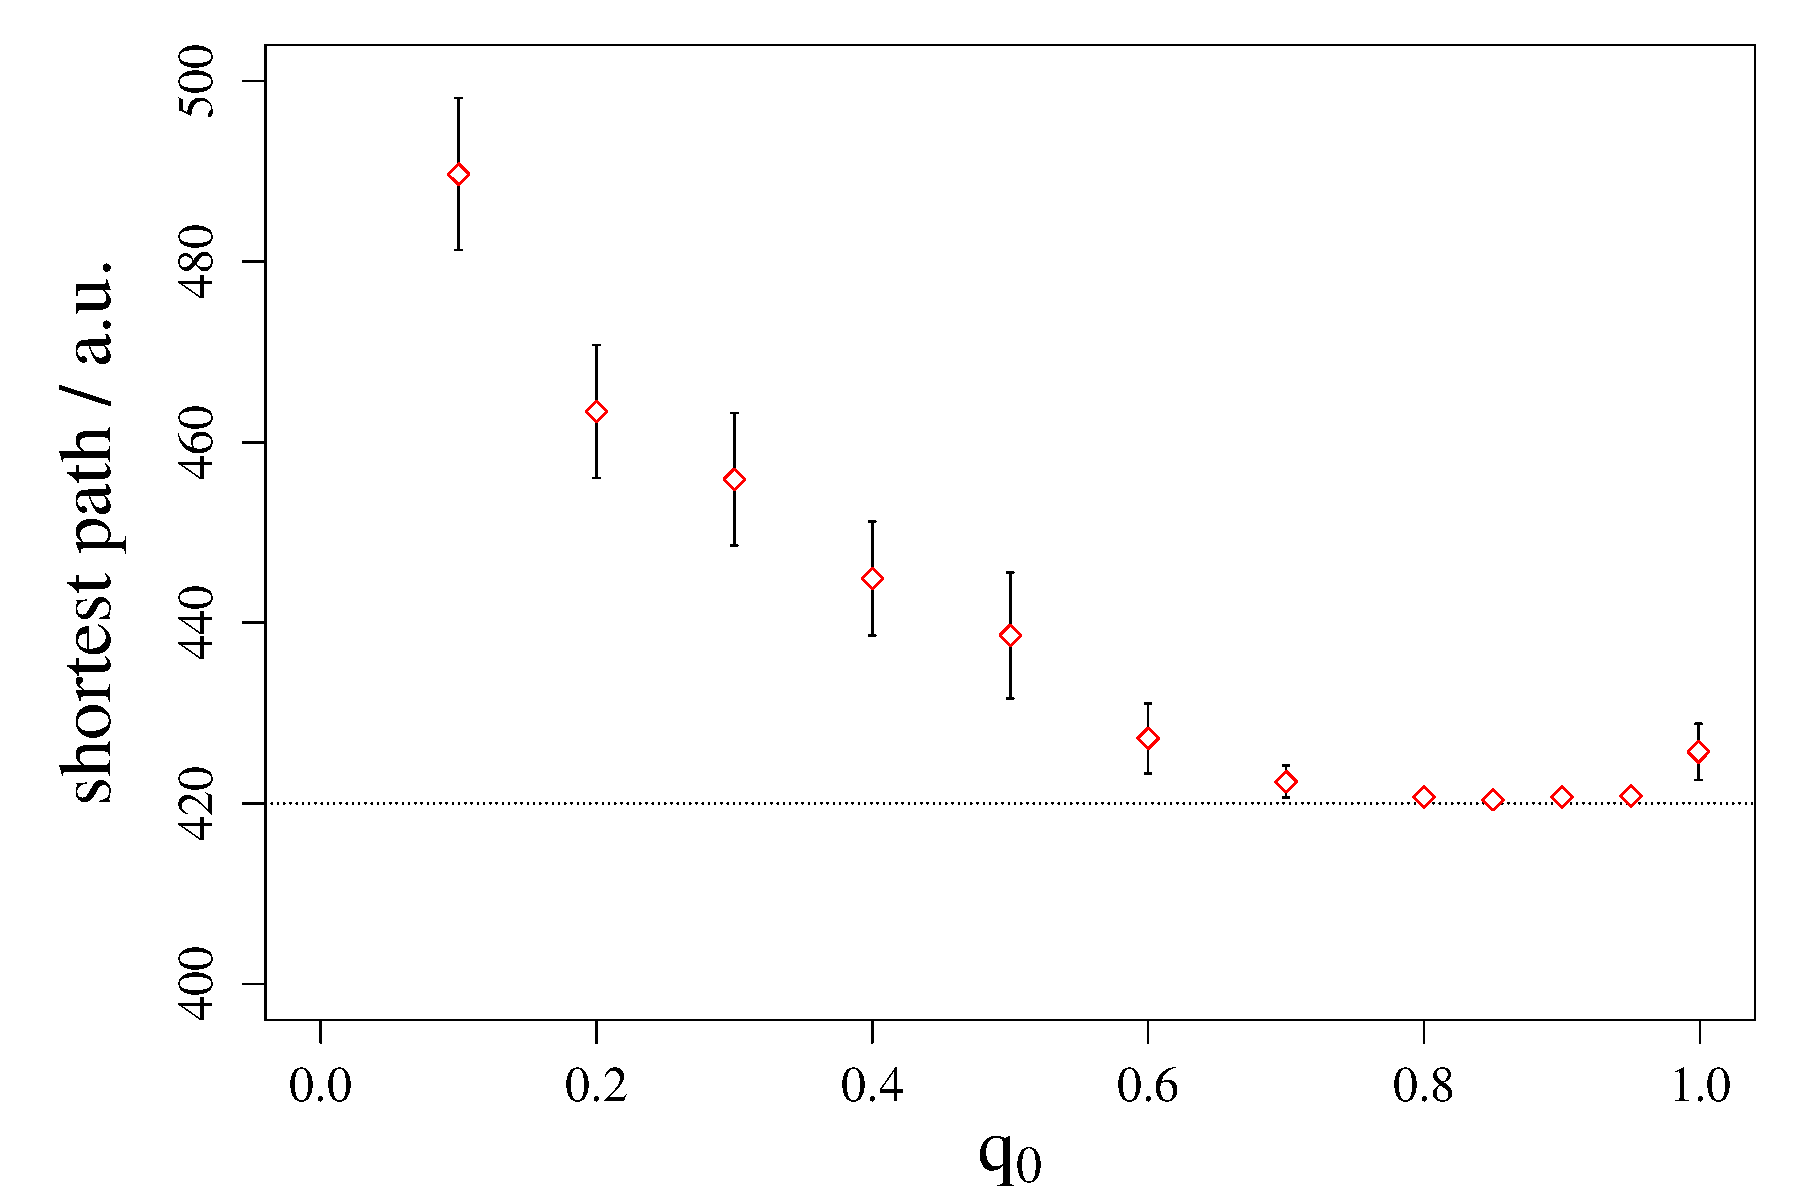
\includegraphics[width=0.8\textwidth]{Plots/q0_vs_shortestpath.pdf}

\caption{The shortest path the simulation found after 800 rounds for the problem \textit{oliver30} is plotted against the probability $q_0$ (see text for impact of $q_0$). The optimal path is shown as a dotted line along with error bars of the data. If no error bars are visible then the errors are smaller then the extent of the points.}
\label{fig:q0zushortestpath}
\end{figure}
